\vspace{-0.2in}
\section{Introduction}
The integration of Large Language Models (LLMs) into scientific discovery \cite{ai4research-survey,agent-laboratory,ai-scientist,scimaster,ai-researcher} has catalyzed a paradigm shift, enabling the generation of research ideas at an unprecedented scale \cite{can-llm-gen-novel,researchagent,chain-of-ideas,alphaevolve}.
However, this ``generative explosion'' has outpaced our evaluative capability, creating a critical bottleneck at the very outset of the research pipeline.
Current innovation evaluation remains heavily dependent on scarce and highly specialized human experts, which is not only time-consuming and costly, but its inherent subjectivity and limited scope also risk overlooking potentially high-value ideas.
Consequently, developing an automated, systematic, and yet human-expert-level idea evaluation framework has become an urgent necessity.

\begin{figure*}
    \centering
    \vskip -0.1cm
    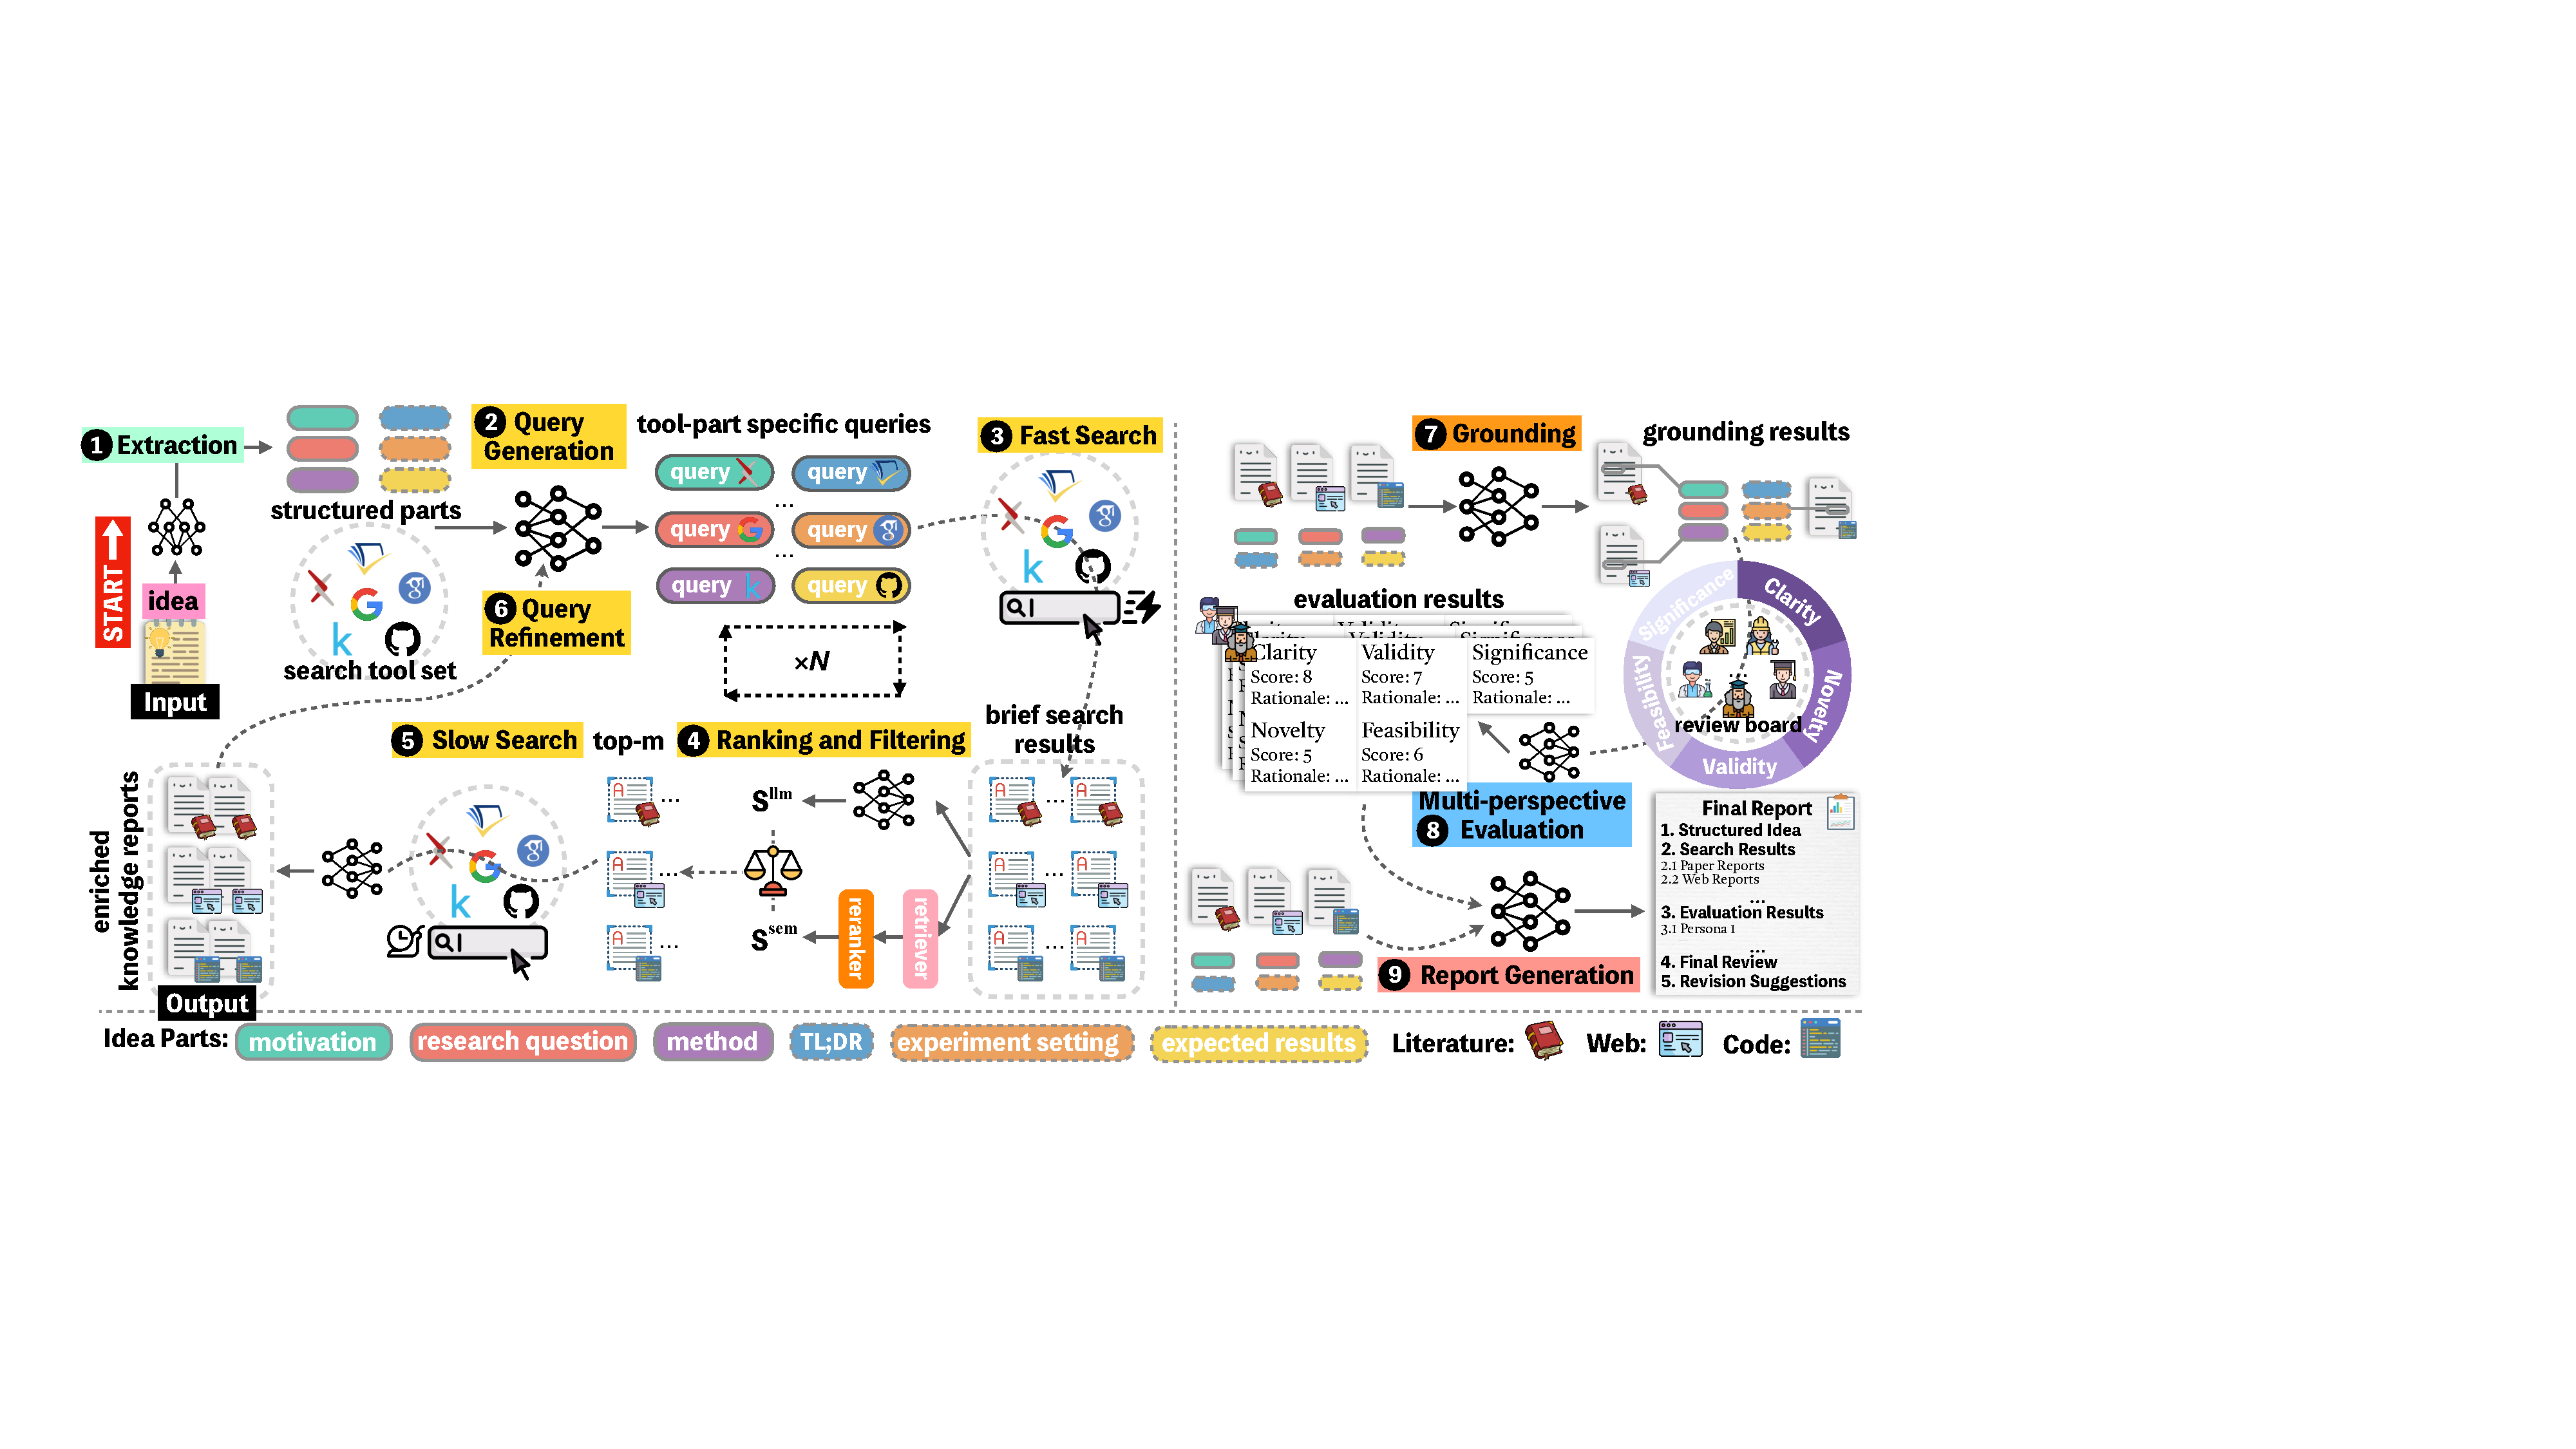
\includegraphics[width=1.\textwidth]{figure/method.pdf}
    \vskip -0.05in
    \caption{\textbf{Framework of {\ours}}. Structured idea parts with dashed boxes are optional. Given the raw-text idea, the deep knowledge search engine (left-hand) iterates $\boldsymbol{N}$ times, ultimately yielding enriched knowledge reports categorized into three types: literature, web, and code. During evaluation, each metric is assessed by a dedicated evaluator agent, and users can freely register additional metrics.}
    \label{fig:method}
    \vskip -0.2in
\end{figure*}

To address this, we must first revisit the fundamental nature of scientific evaluation. Ideally, evaluating a research idea is not a static generation task, but a holistic epistemic verification process, which can be intrinsically defined by three cardinal principles: \textbf{(i) Knowledgeable Grounding} \cite{i-1,i-2}, where idea is a knowledge-intensive entity cross-referenced against the entire living ecosystem of theory and practice; \textbf{(ii) Collective Deliberation} \cite{ii-1,ii-2}, where the quality of assessment emerges from the fusion of diverse expert perspectives, not a single authority; \textbf{(iii) Multi-criteria Decision Making} \cite{iii-1}, where an idea's inherent complexity is honored through the union of multifaceted attributes (e.g., novelty, feasibility, impact) rather than the compression into one or two dimensions.

However, achieving the above principles confronts several challenges that together constitute the core gap between current automated idea evaluation tools \cite{scholareval,opennovelty,litllms,grapheval,idea-novel-checker} and an ideal evaluation system.
First is the \textbf{(i) \textit{narrowness of knowledge horizon}}.
Existing methods are largely confined to static academic papers, overlooking the complete ecosystem of research innovation.
This neglect of ``living knowledge'' renders evaluations divorced from practical realities.
Second is the \textbf{(ii) \textit{overlook of review consensus}}.
Mainstream approaches directly using LLM-as-a-Judge fossilize the models' inherent biases into de facto evaluation criteria, failing to emulate the deliberation among distinct perspectives.
Last is the \textbf{(iii) \textit{flattening of evaluation dimensions}}.
Existing methods typically obscure the independence and internal tensions among multiple attributes embedded in a complete research idea, fail to deliver useful feedback, and violate the multi-criteria decision-making that systematic scientific evaluation should adhere to.

In response to these challenges, we regard idea evaluation as a knowledge-grounded,
multi-perspective reasoning problem and introduce \textbf{\ours}, a deep innovation evaluation framework that emulates the full scholarly review process performed by human experts.
To counter the narrowness of knowledge horizons, we design a \textbf{(i) \textit{heterogeneous deep knowledge search engine}}, which can concurrently obtain living knowledge from online literature, web opinions, and code repos, combining fast search with slow reading for both effectiveness and efficiency.
Through multi-round query refinement and hybrid scoring that blends semantic similarity with LLM judgment, it filters highly relevant, high-quality background knowledge from diverse sources, thereby constructing a living, comprehensive, and cross-domain evidential knowledge base for grounding and evaluation.
Next, to achieve review consensus, we simulate an \textbf{(ii) \textit{innovation review board}} to perform multi-perspective evaluation by sampling multiple reviewers with distinct backgrounds, expertise, and preferences from a carefully curated academic persona pool.
We partially mask the searched knowledge according to each reviewer's role to simulate real human cognition.
Each reviewer will independently judge the research idea, thereby mitigating the bias inherent in a single judge.
During actual evaluation, to overcome flattened evaluation dimensions, we perform a \textbf{(iii) \textit{multi-dimensional decoupled evaluation}}, supporting customizable multi-criteria assessment initialized across five dimensions: \textit{Clarity}, \textit{Novelty}, \textit{Feasibility}, \textit{Validity}, and \textit{Significance}. Each dimension is assessed by a specialized evaluator agent that conducts in-depth analyses grounded in both retrieved heterogeneous knowledge and its own internal knowledge.
All multi-dimensional evaluations from the personified reviewers are aggregated into an actionable report that provides cited knowledge evidence, structured evaluation analyses and scores, a meta-review with specific decisions, and concrete directions for further improvement.

To evaluate {\ours}, we extract real-world ideas from authoritative peer-reviewed papers and construct datasets that respectively inspect single-idea evaluation, pairwise-idea comparison, and group-idea ranking capabilities.
Quantitatively, {\ours} outperforms the strongest baseline by 16.18\% F1 score in three-class point-wise prediction, by roughly 5\% accuracy in pair-wise comparison, and by 7.56\% accuracy in group-wise ranking.
Qualitatively, evaluation reports produced by {\ours} achieve a win rate exceeding 70\% against all baselines in \textit{Overall Quality}.
In human evaluation, {\ours}'s scores exhibit high correlation with human judgments across all metrics.
Further ablation studies confirm the effectiveness of each of our proposed modules.
Exploratory analyses reveal that {\ours}'s evaluation exhibits patterns and phenomena aligned well with human cognition, indicating that it can faithfully simulate the real process of human innovation evaluation.